\documentclass{article}
\usepackage[top=2.5cm, left=3cm, right=3cm, bottom=4.0cm]{geometry}
\usepackage{graphicx} 
\usepackage{amsfonts,amsmath,amssymb}
\usepackage{array}
\usepackage{tabularray}
\usepackage[utf8]{inputenc}
\usepackage[T1]{fontenc}
\usepackage{csquotes}
\usepackage{alphabeta}
\usepackage{url}
\usepackage{hyperref}
\usepackage{esint}

\renewcommand{\figurename}{Γράφημα}

\begin{document}
\begin{table}[ht]
    \begin{tblr}{
        @{}X[l, valign=b]X[c, valign=b]X[r, valign=b]@{}
    }

    \hline
    % First line, course info
    \SetCell[c=2]{l}{[ΘΠ04] Παράλληλα Συστήματα} & & {2024-25} \\ 
    \hline
    {} & {} & {} \\

    % Title
    \SetCell[c=3]{c}{ \Large \textbf{Εργασία 2 - Προγραμματισμός με OpenMP} } \\
    {} & {} & {} \\

    % Name Surname, Student ID
    \hline
    \SetCell[c=3]{c}{ \textbf{Ονοματεπώνυμο:} Μάριος Γιαννόπουλος } \\
    \SetCell[c=3]{c}{ \textbf{A.M.:} 1115200000032} \\
    \hline

    \end{tblr}
\end{table}
\section*{Γενικές Πληροφορίες}

\subsection*{Υπολογιστικό Σύστημα}
Όλο το έργο υλοποιήθηκε στο ίδιο υπολογιστικό περιβάλλον:
\begin{itemize}
    \item \textbf{Όνομα Υπολογιστικού Συστήματος:} Linux12
    \item \textbf{Επεξεργαστής:} Intel(R) Core(TM) i5-6500 CPU @ 3.20GHz
    \item \textbf{Αριθμός Πυρήνων:} 4
    \item \textbf{Λειτουργικό Σύστημα:} Linux Ubuntu 20.04.2 LTS
    \item \textbf{Έκδοση Μεταγλωττιστή:} gcc (Ubuntu 9.4.0-1ubuntu1~20.04.2) 9.4.0
\end{itemize}

\subsection*{Οδηγίες Εκτέλεσης Python Scripts}
Για την εκτέλεση των Python scripts που επεξεργάζονται τα αποτελέσματα, ακολουθήστε τα εξής βήματα:
\begin{enumerate}
    \item Μεταβείτε στον φάκελο \path{scripts}.
    \item Εγκαταστήστε τις απαραίτητες βιβλιοθήκες:
    \begin{verbatim}
    pip install -r requirements.txt
    \end{verbatim}
    \item Εκτελέστε το script που σας ενδιαφέρει:
    \begin{verbatim}
    python <test_script>.py
    \end{verbatim}
\end{enumerate}
\textbf{Σημείωση:} Όλα τα αποτελέσματα στα γραφήματα είναι από την εκτέλεση των πειραμάτων στο εργαστήριο Linux. Κάθε πείραμα εκτελέστηκε 5 φορές και τα αποτελέσματα αναφέρονται στο μέσο όρο των επαναλήψεων.
\section*{Άσκηση 2.1}
\subsection*{Εισαγωγή}
Σκοπός της παρούσας εργασίας είναι η παραλληλοποίηση του Παιχνιδιού της Ζωής (Game of Life) με χρήση της βιβλιοθήκης OpenMP. Το παιχνίδι, που σχεδιάστηκε από τον John Conway το 1970, είναι ένα μαθηματικό μοντέλο τοπικών κανόνων που παράγει πολύπλοκα μοτίβα. Στο πλαίσιο της εργασίας, υλοποιήθηκε τόσο σειριακή όσο και παράλληλη έκδοση του αλγορίθμου, ενώ τα πειράματα εκτελέστηκαν σε διαφορετικά μεγέθη πλεγμάτων και αριθμούς νημάτων.

\subsection*{Συγχρονισμός}
Για την υλοποίηση της παράλληλης έκδοσης, χρησιμοποιήθηκαν οι διευθύνσεις OpenMP για την κατανομή του έργου στα διαθέσιμα νήματα. Λόγω της φύσης της εφαρμογής, κάθε γενιά ενημερώνεται ταυτόχρονα, οπότε δεν απαιτήθηκε πρόσθετος συγχρονισμός μεταξύ των νημάτων.

\subsection*{Πειραματική Διαδικασία}
\begin{itemize}
    \item \textbf{Παραμετροποίηση:}
    \begin{itemize}
        \item Μέγεθος πλέγματος: $64 \times 64$, $1024 \times 1024$, $4096 \times 4096$.
        \item Αριθμός γενιών: 1000.
        \item Αριθμός νημάτων: 2, 4, 8, 16.
    \end{itemize}
    \item \textbf{Εκτέλεση:}
    \begin{itemize}
        \item Τα πειράματα εκτελέστηκαν 5 φορές για κάθε συνδυασμό παραμέτρων.
        \item Καταγράφηκε ο χρόνος εκτέλεσης για κάθε πείραμα.
        \item Τα δεδομένα αποθηκεύτηκαν σε CSV αρχείο.
    \end{itemize}
    \item \textbf{Αυτοματοποίηση:}
    \begin{itemize}
        \item Αναπτύξαμε Python scripts για την εκτέλεση των πειραμάτων και την καταγραφή των δεδομένων.
        \item Χρησιμοποιήθηκαν Python scripts για την επεξεργασία των αποτελεσμάτων και τη δημιουργία γραφημάτων.
    \end{itemize}
\end{itemize}

\subsection*{Αποτελέσματα}
\begin{itemize}
    \item \textbf{Σύγκριση Σειριακού και Παράλληλου Αλγορίθμου:}
    \begin{itemize}
        \item Για μικρά πλέγματα ($64 \times 64$), η σειριακή έκδοση ήταν ταχύτερη λόγω του overhead της παραλληλοποίησης.
        \item Για μεγαλύτερα πλέγματα ($1024 \times 1024$ και $4096 \times 4096$), ο παράλληλος αλγόριθμος απέδωσε καλύτερα.
    \end{itemize}
    \item \textbf{Επιτάχυνση:}
    \begin{itemize}
        \item Η ταχύτητα εκτέλεσης βελτιώθηκε σημαντικά με την αύξηση του αριθμού των νημάτων, μέχρι να φτάσει το όριο των πυρήνων του επεξεργαστή.
        \item Το μέγεθος του πλέγματος επηρέασε σημαντικά την απόδοση της παραλληλοποίησης.
    \end{itemize}
\end{itemize}
% \subsection*{Γραφήματα}
% Το παρακάτω γράφημα παρουσιάζει τη σχέση μεταξύ του μεγέθους του πλέγματος, του αριθμού των νημάτων και του χρόνου εκτέλεσης:
% \begin{figure}[h]
%     \centering
%     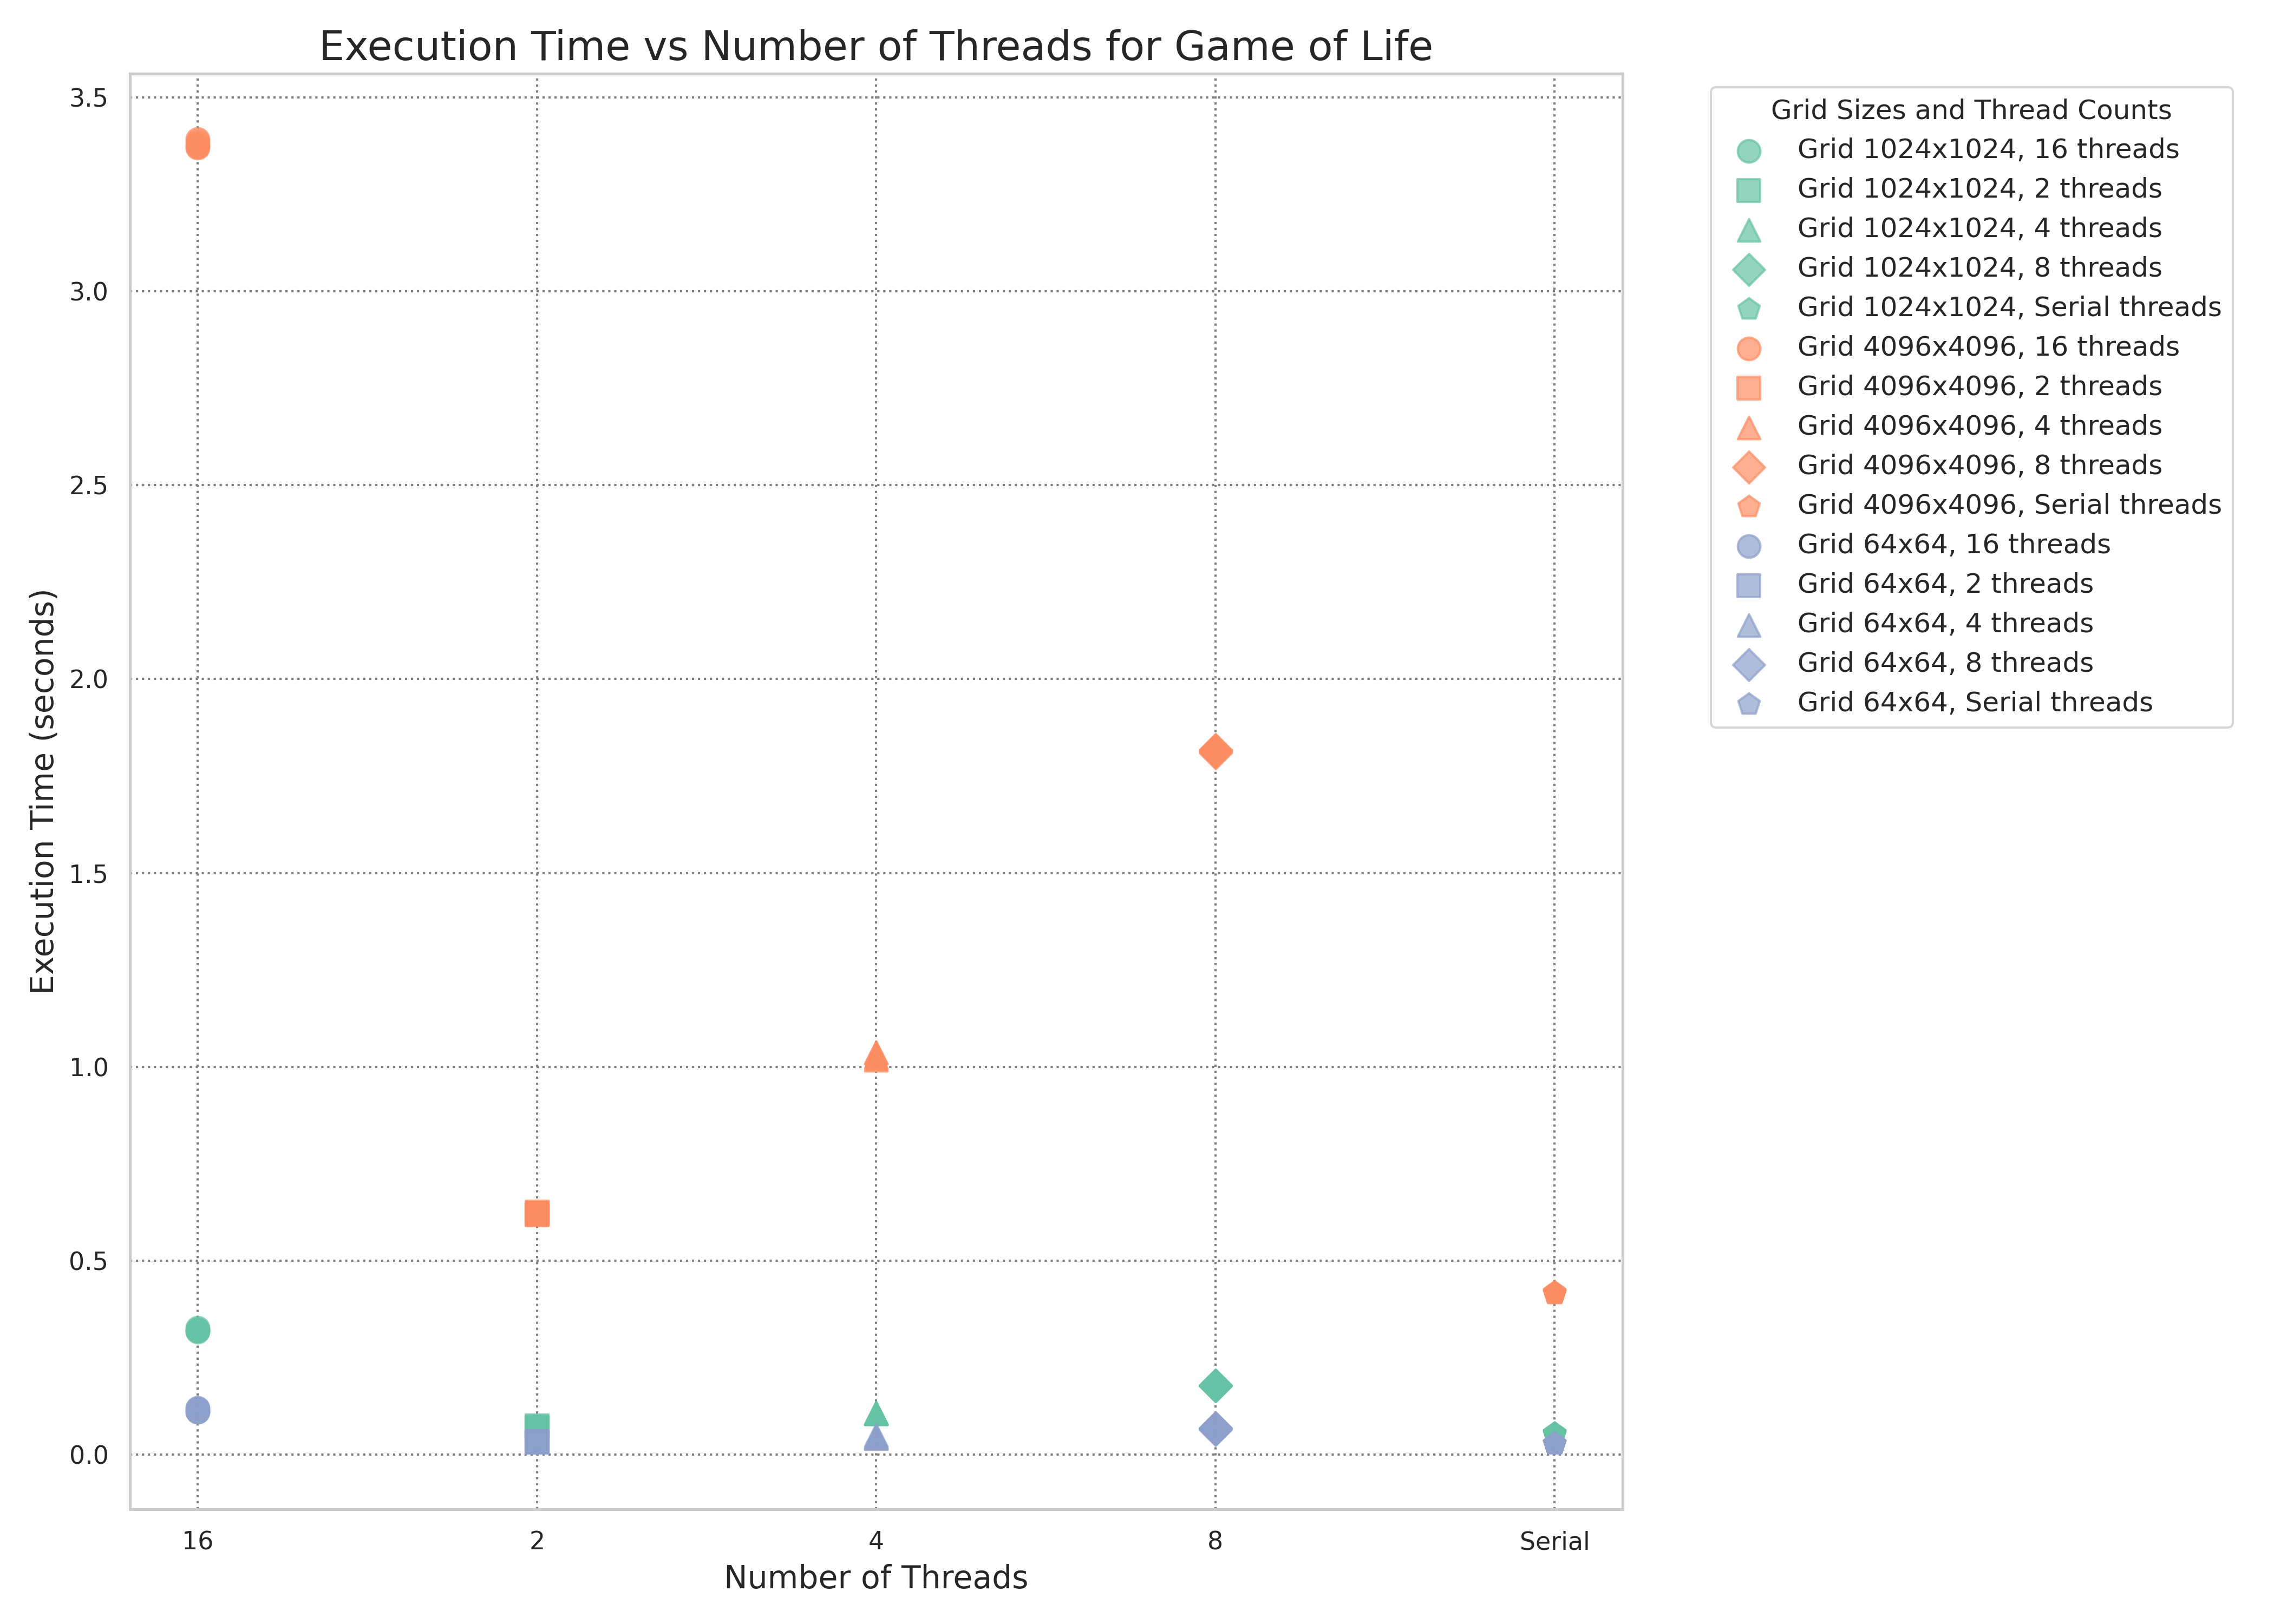
\includegraphics[width=1\textwidth]{game_of_life_results.png}
%     \caption{Χρόνος Εκτέλεσης ανά Μέγεθος Πλέγματος και Αριθμό Νημάτων}
% \end{figure}
\subsection*{Συμπεράσματα}
\begin{enumerate}
    \item Η παραλληλοποίηση είναι αποδοτική για μεγάλα μεγέθη πλεγμάτων.
    \item Η απόδοση του αλγορίθμου περιορίζεται από τον αριθμό των διαθέσιμων πυρήνων.
    \item Για μικρά μεγέθη πλεγμάτων, η σειριακή έκδοση παραμένει αποδοτικότερη λόγω του overhead της παραλληλοποίησης.
\end{enumerate}
Η εργασία κατέδειξε τη σημασία της παραλληλοποίησης για μεγάλα προβλήματα, αλλά και τους περιορισμούς της λόγω του hardware.
\section*{Άσκηση 2.2}
\subsection*{Εισαγωγή}
Η παρούσα εργασία εξετάζει την παραλληλοποίηση της διαδικασίας επίλυσης γραμμικών συστημάτων με τη χρήση της απαλοιφής Gauss και της αντικατάστασης προς τα πίσω. Η απαλοιφή Gauss μετατρέπει ένα σύστημα σε άνω τριγωνική μορφή, ενώ η αντικατάσταση προς τα πίσω υπολογίζει τις λύσεις. Η εργασία περιλαμβάνει σειριακές και παράλληλες υλοποιήσεις τόσο για τον «κατά γραμμή» όσο και για τον «κατά στήλη» αλγόριθμο. Η αξιολόγηση των υλοποιήσεων γίνεται μέσω πειραμάτων σε διάφορα μεγέθη συστημάτων και αριθμούς νημάτων.
\subsection*{Πειραματική Διαδικασία}
\subsection*{Αποτελέσματα}
\subsection*{Γραφήματα}
\subsection*{Συμπεράσματα}
Η εργασία ανέδειξε την αποδοτικότητα της παραλληλοποίησης για μεγάλα συστήματα, ενώ τόνισε τη σημασία της βέλτιστης χρήσης των εργαλείων OpenMP για τη μέγιστη αξιοποίηση του hardware.
\section*{Άσκηση 2.3}
\subsection*{Εισαγωγή}
\subsection*{Πειραματική Διαδικασία}
\subsection*{Αποτελέσματα}
\subsection*{Γραφήματα}
\subsection*{Συμπεράσματα}
\end{document}